\begin{frame}{Diagonalizable matrices}
\begin{definition}
An $n\times n$ matrix $A$ is {\bf diagonalizable} if there is an invertible matrix $P$ such that $D=P^{-1}AP$ is diagonal. 

In other words, $A$ is diagonalizable if it is \alert{similar} to a diagonal matrix $D$. 
\end{definition}
 \pause
 \begin{comments}
 \bb
 \ii If $A$ is itself diagonal, then it is diagonalizable: we may choose $P=I_n$ in the definition. 
 \pause\ii In this section we will develop a systematic procedure for determining whether a matrix is diagonalizable. As we will see, the answer is yes if and only if $A$ has ``enough" linearly independent eigenvectors. Of course we will spell out precisely what we mean by ``enough". 
 \pause\ii Not all matrices are diagonalizable. For example, $A=\begin{bmatrix}
 0&1\\
 0&0
 \end{bmatrix}$ is not diagonalizable, as the aforementioned procedure will show. 
 \pause\ii Roughly speaking, you should interpret being diagonalizable as meaning ``as good as diagonal". To elaborate: doing arithmetic with diagonal matrices $D$ is extremely easy; if we know $A$ is diagonalizable, meaning it is similar to a diagonal matrix $D$, then it shares many essential properties of $D$, and we can use the relation $D=P^{-1}AP$ to help ease arithmetic computations involving $A$.   \ee
 \end{comments}
\end{frame}
\begin{frame}{Properties of conjugation}
If we have, $D=P^{-1}AP$, why exactly is there such a close connection between $D$ and $A$? One explanation has to do with the underlying operation  
\[
A\longmapsto P^{-1}AP,
\]
which we call \alert{conjugation by $P$}.  As the following theorem outlines, conjugation by an invertible $P$ satisfies many useful properties, and we use these to relate the matrix $A$ with the matrix $P^{-1}AP$. 
\pause
\begin{theorem}[Properties of conjugation]\label{th:conjugation}
Let $P$ be any invertible $n\times n$ matrix. 
\bb
\ii $P^{-1}(c_1A_1+c_2A_2)P=c_1P^{-1}A_1P+c_2P^{-1}A_2P$. (\alert{Conjugation by $P$ is a linear transformation}.) 
\ii $P^{-1}A^nP=(P^{-1}AP)^n$ for any integer $n\geq 0$. If $A$ is invertible, the equality holds for {\em all} integers $n$. (\alert{Conjugation preserves powers}.) 
\ii Recall that given any polynomial $f(x)=\anpoly$ and any $n\times n$ matrix $A$ we define $f(A)=a_nA^n+a_{n-1}A^{n-1}+a_1A+a_0I_n$. 

We have $f(P^{-1}AP)=P^{-1}f(A)P$ for any polynomial $f(x)$, and any $n\times n$ matrix $A$. (\alert{Conjugation preserves polynomial evaluation}.) 
\ee
\end{theorem}
\pause
\begin{proof}
Exercise.
\end{proof}
\end{frame}
\begin{frame}{Examples: utility of diagonalizability}
Suppose $A$ is diagonalizable, so that $D=P^{-1}AP$, where $D$ is diagonal with diagonal entries $d_i$. Using Theorem \ref{th:conjugation}, we can now see how to translate statements about $D$ (which are generally easy to prove), to statements about $A$ (which otherwise might have been difficult to show). 
\begin{example}\label{eg:diagpowers}
To compute $A^{n}$ (hard) we can just compute $D^{n}$ (easy) and then observe that $A=PDP^{-1}$, and thus 
\[
A^{n}=(PDP^{-1})^{n}=PD^{n}P^{-1},
\] 
where the last equality follows from part (b) of Theorem \ref{th:conjugation}; here we let $P^{-1}$ assume the role of $P$ in the theorem statement. 
\bpause
For example, let $A=\begin{bmatrix}
1&3\\
1&-1
\end{bmatrix}$. Let's compute $A^n$ for arbitrary $n$. 

We have $D=P^{-1}AP$, where $D=\begin{bmatrix}[rr]
2&0\\
0&-2
\end{bmatrix}$, and $P=\begin{bmatrix}[rr]
3&1\\
1&-1
\end{bmatrix}$. (This is not obvious yet. Soon we will have the tools to see why this is so.)
\bpause 
Then $A=PDP^{-1}$, and thus 
\[
A^{n}=PD^{n}P^{-1}=P\begin{bmatrix}
2^{100}&0\\
0&(-2)^{100}
\end{bmatrix}P^{-1}=\frac{1}{4}\begin{bmatrix}
3\cdot2^n+(-2)^n&3\cdot 2^n-3(-2)^{n}\\
2^{n}-(-2)^n&2^n+3(-2)^{n}
\end{bmatrix}.
\] 
\end{example}

\end{frame}
\begin{frame}{Examples: utility of diagonalizability}
Suppose $A$ is diagonalizable, so that $D=P^{-1}AP$, where $D$ is diagonal with diagonal entries $d_i$. 
\begin{example}
More generally, we have $f(A)=f(PDP^{-1})=Pf(D)P^{-1}$ for any polynomial $f(x)=\anpoly$. Since $D$ is diagonal, with diagonal entries $d_i$, it is easy to see that $f(D)$ is also diagonal, with diagonal entries $f(d_i)$. 
\bpause
In particular we see that $f(A)=\underset{n\times n}{\boldzero}$ if and only if $f(D)=\underset{n\times n}{\boldzero}$, and this holds if and only if $f(d_i)=0$ for each diagonal entry $d_i$ of $D$.  
\bpause
Take the matrix $A$ from Example \ref{eg:diagpowers}, and let $f(x)=(x-2)(x+2)=x^2-4$. Since $f(2)=f(-2)=0$, it follows that $f(D)=f(A)=\underset{2\times 2}{\boldzero}$. In other words, $A^2-4I=\underset{2\times 2}{\boldzero}$, as you can easily check. 

\end{example}
\end{frame}
\begin{frame}{Examples: utility of diagonalizability}
Suppose $A$ is diagonalizable, so that $D=P^{-1}AP$, where $D$ is diagonal with diagonal entries $d_i$. 
\begin{example}
$A$ has a \alert{square-root} (i.e., a matrix $B$ such that $B^2=A$) iff $D$ has a square-root. 
\bpause Indeed, suppose $B^2=A$. Set $C=P^{-1}BP$. Then $C^2=P^{-1}B^2P=P^{-1}AP=D$. Similarly, if $C^2=D$, then $B^2=A$, where $B=PCP^{-1}$. 
\bpause
As an example,  the matrix $A=\begin{bmatrix}
0&-2\\
1 &3
\end{bmatrix}$, satisfies $D=P^{-1}AP$, where $D=\begin{bmatrix}
1&0\\
0&2
\end{bmatrix}$, and $P=\begin{bmatrix}
2&1\\
-1&-1
\end{bmatrix}$. Since $C=\begin{bmatrix}
1&0\\
0&\sqrt{2}
\end{bmatrix}$ is a square-root of $D$, $B=PCP^{-1}=\begin{bmatrix}
2-\sqrt{2}&2-2\sqrt{2}\\
-1+\sqrt{2}&-1+2\sqrt{2}
\end{bmatrix}$ is a square-root of $A$, as you can easily check. 
\bpause
So when exactly does a diagonal matrix $D$ have a square-root? Clearly, it is sufficient that $d_i\geq 0$ for all $i$, as in the example above. Interestingly, this is not a necessary condition! Indeed, consider the following example: 

$
\begin{bmatrix}[rr]
-1&0\\
0&-1
\end{bmatrix}=\begin{bmatrix}[rr]
0&-1\\
1&0
\end{bmatrix}^2.
$ 
\end{example}
\end{frame}

\begin{frame}{Properties of similarity}
Before investigating the question of when a matrix is diagonalizable, we record a few more properties illustrating the close connection between similar matrices. 
\begin{theorem}[Properties of similarity]\label{th:similarity}
Suppose $A$ is similar to $B$: i.e., there is an invertible matrix $P$ such that $B=P^{-1}AP$. Then:
\bb[(a)]
\ii $B$ is similar to $A$. (\alert{Similarity is symmetric}.)
\ii $A$ and $B$ have the same trace and determinant. 
\ii $A$ and $B$ have the same rank. 
\ii $A$ and $B$ have the same characteristic polynomial.  
\ii $A$ and $B$ have the same eigenvalues. 
\ii Given any $\lambda\in\R$, let $W_\lambda$ be the corresponding eigenspace for $A$, and $W_\lambda'$ the corresponding eigenspace for $B$. Then $\dim W_{\lambda}=\dim W_{\lambda}'$. 
\ee
\end{theorem}
\pause The proof of (d) follows. I leave the rest as an exercise. 
\end{frame}
\begin{frame}
\begin{proof}[Proof of Theorem \ref{th:similarity}.d]
By definition we have $B=P^{-1}AP$ for some matrix $P$. We wish to show the characteristic polynomials $p_A(t)$ and $p_B(t)$ of the two matrices are equal. Compute:  
\begin{eqnarray*}
p_B(t)&=&\det(tI-B)\\
\pause &=&\det(tI-P^{-1}AP) \\
\pause &=&\det(tP^{-1}IP-P^{-1}AP) \ \text{ (since $P^{-1}IP=I$)} \\
\pause &=&\det(P^{-1}tIP-P^{-1}AP) \ \text{ ($t$ behaves as scalar)} \\
\pause &=&\det(P^{-1}(tI-A)P) \\
\pause &=&\det(P^{-1})\det(tI-A)\det(P)\\
\pause &=&(\det(P))^{-1}\det(P)\det(tI-A)\\
\pause &=&\det(tI-A)=p_A(t). 
\end{eqnarray*}
\end{proof}
\end{frame}
\begin{frame}{The true meaning of similarity}
Hopefully Theorems \ref{th:conjugation} and \ref{th:similarity} convince you that similar matrices (in the linear algebraic sence) are truly similar (in the usual sense). 
\bpause
There is, however, a deeper explanation for this. Namely, if $A$ and $A'$ are similar, then they are simply two different matrix representations of a common linear transformation!
\pause

In more detail: suppose we have $A'=P^{-1}AP$. 
\begin{itemize}
\ii Let $B$ be the standard basis of $\R^n$, and let $B'$ be the basis of $\R^n$ obtained by taking the columns of the invertible matrix $P$. Finally, let $T=T_A$ be the matrix transformation associated to $A$. 
\ii Then $A=[T]_B$, $P=\underset{B'\rightarrow B}{P}$, and $P^{-1}=\underset{B\rightarrow B'}{P}$. 
\ii From the change of basis formula it follows that 
\[
A'=P^{-1}AP=\underset{B\rightarrow B'}{P}[T]_B\underset{B'\rightarrow B}{P}=[T]_{B'}
\]
\end{itemize}
\bpause
In other words to say $A$ and $A'$ are similar is simply to say that they are different matrix representations of the same overlying linear transformation $T$ (see Holy Commutative Tent of Linear Algebra on next slide). All their shared properties (same eigenvalues, same determinant, same trace, etc.) are simply the properties they inherit from this one overlying $T$, of which they are but earthly shadows. 
\bpause
There is one true $T$!
\end{frame}
\begin{frame}
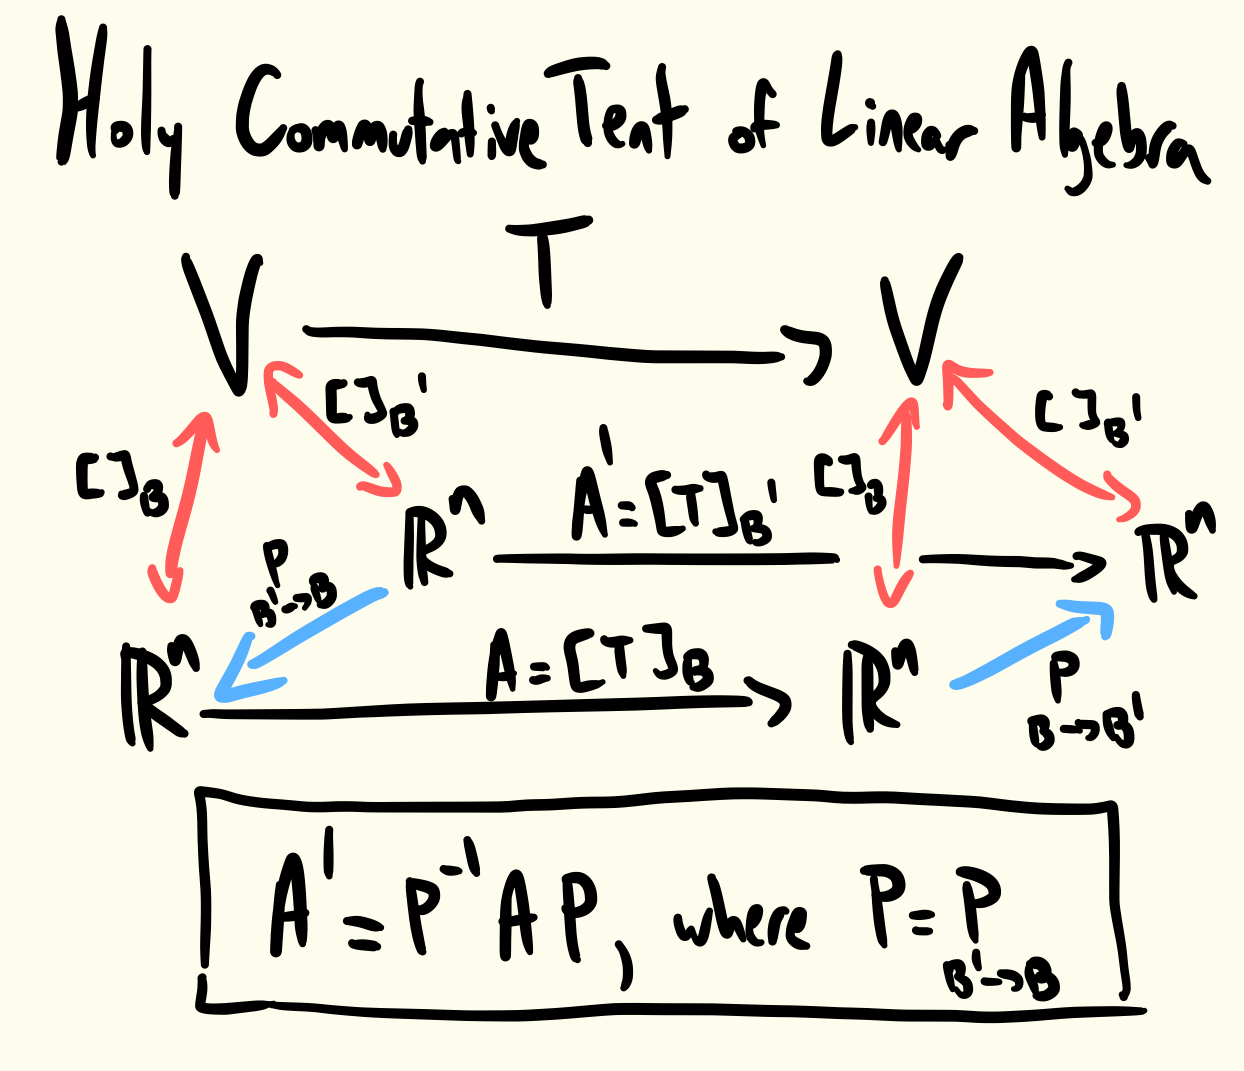
\includegraphics[width=4.5in]{Images/HolyCommutativeTent}

\end{frame}

%\begin{frame}
%\alert{Theorem (Holy commutative tent of linear algebra)}
%The following statements are equivalent:
%
%\alert{(i)} $A$ and $A'$ are similar. 
%
%\alert{(ii)} There is a linear $T\colon V\rightarrow V$ and bases $B$, $B'$ of $V$ such that $A=[T]_B$, $A'=[T]_{B'}$. 
%
%Furthermore, in this situation we have $A'=P^{-1}AP$, where $P=\underset{B'\rightarrow B}{P}$. 
%\pause
%\begin{proof}
%\alert{(ii)$\Rightarrow$ (i)}. 
%Suppose $A=[T]_B$ and $A'=[T]_{B'}$ are two different matrix representations of $T$. Then 
%the change of basis for transformations theorem ( \ref{Th:changeofbasis}) tells us that 
%$
%A'=(P_{B' \rightarrow B})^{-1}AP_{B' \rightarrow B}.
%$
%Thus $A$ and $A'$ are similar. 
%
%\bpause
%\alert{(i)$\Rightarrow$(ii)}. 
%Suppose $A=P^{-1}A'P$. Set $T=T_{A}$, let $B$ be the standard basis of $\R^n$ and let $B'$ be the basis we get by taking the columns of $P$. Then $P=\underset{B'\rightarrow B}{P}$ and $P^{-1}=\underset{B\rightarrow B'}{P}$. 
%
%It is clear with this setup that $A=[T]_B$, since $B$ is the standard basis. Using the relation $A'=P^{-1}AP$ and the  change of basis for transformations theorem ( \ref{Th:changeofbasis}), we have $A'=[T]_{B'}$. 
%\end{proof}
%\end{frame}
\begin{frame}
\footnotesize
The previous theorem allows us to extend some of our matrix definitions to linear transformations. 
\begin{definition}
Let $T\colon V\rightarrow V$ be linear, let $B$ be \alert{any basis} of $V$, and let $A=[T]_B$. We  define
the {\bf characteristic polynomial} of $T$ to be $p(t)=\det(tI-A)$. 
\end{definition}
\pause
\begin{comment}
Note that the characteristic polynomial defined above does not depend on the choice of basis $B$. If $B'$ is another basis, and $A'=[T]_{B'}$, then $A'$ and $A$ are similar, as we have seen, and thus have the same characteristic polynomial. 
\end{comment}
\pause
\begin{definition}
A linear transformation $T\colon V\rightarrow V$ is {\bf diagonalizable} if there exists a basis $B$ of $V$ for which $[T]_B$ is a diagonal matrix. 
\end{definition}
 \pause
 \begin{comment}
Equivalently, $T$ is diagonalizable if for \alert{any} choice of basis $B$ the matrix $[T]_B$ is diagonal\alert{izable}.  
 \end{comment}
 \end{frame}
\begin{frame}{Diagonalizability and eigenvectors}
At last we relate the property of being diagonalizable with the notion of eigenvectors. In the process we make clear what we mean when we say $T$ is diagonalizable if and only if it has ``enough" linearly independent eigenvectors. 
\pause
\begin{theorem}[Diagonalizability theorem]\label{th:diagonalizability}
Let $T\colon V\rightarrow V$ be linear, $\dim(V)=n$.
\bb
\ii (\alert{Qualitative}) Given basis $B$ of $V$, the matrix $[T]_B$ is diagonal if and only if $B$ consists of eigenvectors of $T$. 

Thus $T$ is diagonalizable if and only if there is a basis of $V$ consisting of eigenvectors of $T$. 
\ii (\alert{Quantitative}) Let $\lambda_1, \lambda_2, \dots, \lambda_r$ be the \alert{distinct} eigenvalues of $T$, let $W_{\lambda_j}$ be the corresponding eigenspaces, and let $n_j=\dim W_{\lambda_j}$. 

Then $T \text{ is diagonalizable}\Longleftrightarrow n_1+n_2+\cdots +n_r=n$.
\ee
\end{theorem}
\pause
\begin{proof}
The first statement was a homework exercise. The proof of the second statement is within our means, but somewhat lengthy. I will sketch its proof elsewhere.  For now it is more important to understand how to use the result. 
\end{proof}
\end{frame}

\begin{frame}{Deciding whether $T\colon V\rightarrow V$ is diagonalizable}
Suppose $\dim(V)=n$. 
\bb
\ii Pick a basis $B$ of $V$. Set $A=[T]_B$
\pause\ii Find the distinct eigenvalues, $\lambda_1,\dots, \lambda_r$,  of $A$, let $W_{\lambda_i}$ be the corresponding eigenspaces, and let $n_i=\dim W_{\lambda_i}$.
\pause\ii $A$ (and thus $T$) is diagonalizable if and only if 
$
n_1+n_2+\cdots +n_r=n.
$ 
\pause\ii If the above equality is true, compute bases for each $W_{\lambda_i}$ in $\R^n$. 
\pause\ii Lift all vectors from all these bases back to $V$ using $[\hspace{5pt}]_B$. This is a new basis $B'$ of $V$ consisting of eigenvectors of $T$. 
\pause\ii $[T]_{B'}=D$ is diagonal. 
\ee

\end{frame}
\begin{frame}{Deciding whether $A_{n\times n}$ is diagonalizable}
\bb
\ii Find the distinct eigenvalues, $\lambda_1,\dots, \lambda_r$,  of $A$, let $W_{\lambda_i}$ be the corresponding eigenspaces, and let $n_i=\dim W_{\lambda_i}$.
\pause\ii $A$ is diagonalizable if and only if 
$
n_1+n_2+\cdots +n_r=n.
$ 
\pause\ii If the above equality is true, compute bases $B_j$ for each $W_{\lambda_j}$. 
\pause\ii Place all the vectors from the bases $B_j$ as columns of a matrix $P$. As these eigenvectors are linearly independent, $P$ is invertible.  
\pause\ii The matrix $D=P^{-1}AP$ is diagonal. 

In more detail, the $j$-th diagonal entry of $D$ is the eigenvalue associated to the eigenvector in the $j$-th column of $P$. This means the first $n_1$ diagonal entries of $D$ are equal to $\lambda_1$, the next $n_2$ entries are equal to $\lambda_2$, etc. 
\ee

\end{frame}
\begin{frame}{Example}
Take $A=\begin{bmatrix}
1&1\\
0&1
\end{bmatrix}$. Earlier I claimed that this matrix is not diagonalizable. Let's see why.
\bpause
The characteristic polynomial of $A$ is $p(t)=(t-1)^2$. Thus $\lambda=1$ is the only eigenvalue of $A$. 
\bpause
We have $W_1=\NS(I-A)=\NS\begin{bmatrix}
0&-1\\
0&0
\end{bmatrix}$. We see clearly that $\rank(I-A)=1$, and hence $\dim W_1=\dim\NS(I-A)=2-1=1$. 
\bpause
Since $W_1$ is the only eigenspace, and since $\dim W_1=1\ne 2$, we conclude $A$ is not diagonalizable. 
\end{frame}
\begin{frame}{Example}
Let $A=\begin{bmatrix}[rrrr]
14 & 21 & 3 & -39 \\
12 & 25 & 3 & -41 \\
12 & 24 & 5 & -42 \\
12 & 22 & 3 & -38
\end{bmatrix}$.  
\bpause
The characteristic polynomial of $A$ is $p(t)=x^4 - 6x^3 + 9x^2 + 4x - 12$. (This is not obvious, but would be a pain to compute in detail. You may take this for granted.) 
\bpause
Our usual factoring tricks allow us to factor this as $p(x)=(x-2)^2(x+1)(x-3)$. 
\bpause
The eigenspaces are $W_2=\NS(2I-A), W_{-1}=\NS(-I-A)$, and $W_3=\null(3I-A)$. I'll leave it to you to verify that they have bases $B=\{ (3,2,0,2), (1,1,2,1)\}$, $B'=\{(1,1,1,1)\}$, and $B''=\{(3,5,6,4)\}$, respectively. 
\bpause
It follows that the dimensions of the eigenspaces are 2, 1, and 1, respectively. Since $2+1+1=4$, we conclude that $A$ is diagonalizable. 
\bpause
In more detail, we have $D=P^{-1}AP$, where 
\[
D=\begin{bmatrix}[rrrr]
2&0&0&0\\
0&2&0&0\\
0&0&-1&0\\
0&0&0&3
\end{bmatrix}, \ \
P=\begin{bmatrix}[rrrr]
3 & 1 & 1 & 3 \\
2 & 1 & 1 & 5 \\
0 & 2 & 1 & 6 \\
2 & 1 & 1 & 4
\end{bmatrix}
\]
\end{frame}

\begin{frame}{Geometric and algebraic multiplicity}
Take $A$ (or $T$) and suppose the characteristic polynomial $p(t)$ factors as 
\[
p(t)=(t-\lambda_1)^{n_1}(t-\lambda_2)^{n_2}\cdots (t-\lambda_r)^{n_r},
\]
where the $\lambda_i$ are the {\em distinct} eigenvalues of $A$ (or $T$). It turns out that the exponent $n_i$, called the {\bf algebraic multiplicity} of the eigenvalue $\lambda_i$, is an upper bound on $m_i=\dim W_{\lambda_i}$, called the {\bf geometric multiplicity}. 
\pause
\begin{theorem}[Algebraic and geometric multiplicity theorem]
Let $A$ (or $T$) have characterisitc polynomial 
\[
p(t)=(t-\lambda_1)^{n_1}(t-\lambda_2)^{n_2}\cdots (t-\lambda_r)^{n_r},
\]
where the $\lambda_i$ are the {\em distinct} eigenvalues of $A$ (or $T$). Then 
\[
\dim W_{\lambda_i}\leq n_i:
\]
i.e., the geometric multiplicity is less than or equal to the algebraic multiplicity. 
\end{theorem}
 
\end{frame}
\begin{frame}{Linear independence and eigenvectors}
The following result is used to prove the diagonalizability theorem (Theorem \ref{th:diagonalizability}), but is also very useful in its own right. 
\begin{theorem}\label{th:independentteigenvectors}
Let $T\colon V\rightarrow V$ be a linear transformation, and let $S=\{\boldv_1,\dots, \boldv_r\}$ be a set of eigenvectors of $T$ with $T\boldv_i=\lambda_i\boldv_i$. 

If the $\lambda_i$ are all distinct, then $S$ is linearly independent. 
\end{theorem}
\pause
\begin{proof}
Proved elsewhere.
\end{proof}
\pause
\begin{corollary}
Let $T\colon V\rightarrow V$ be a linear transformation, and suppose $\dim V=n$. 

If $T$ has $n$ \alert{distinct} eigenvalues, then $T$ is diagonalizable. 
\end{corollary}
\pause
\begin{proof}
Let $\boldv_1, \boldv_2,\dots, \boldv_n$ be eigenvectors corresponding to these $n$ distinct eigenvalues. The theorem tells us they form a linearly independent set. Since $\dim V=n$, they form a basis for $V$ by the dimension theorem compendium. Since $T$ has a basis of eigenvectors, it is diagonalizable. 
\end{proof}

\end{frame}
\begin{frame}
Theorem \ref{th:independentteigenvectors} makes no assumption about the dimension of $V$. It can thus be applied to interesting infinite-dimensional examples. 
\begin{example} 
Let $V=C^\infty(\R)$, and let $T\colon V\rightarrow V$ be defined as $T(f)=f'$. 

Let $f_i(x)=e^{k_ix}$, where the $k_i$ are all distinct constants. I claim $S=\{f_1,f_2,\dots , f_r\}$ is linearly independent. 
\bpause 
Indeed, each $f_i$ is an eigenvector of $T$, since $T(f_i)=(e^{k_ix})'=k_ie^{k_ix}=k_if_i$. 
\bpause 
Since the $k_i$'s are all distinct, it follows that the $f_i$ are eigenvectors with distinct eigenvalues, hence linearly independent!

\pause Note: try proving that $S$ is linearly independent using the the Wronskian! You get a very interesting determinant computation.  
\end{example}
\end{frame}
%\begin{frame}{Conditions guaranteeing diagonalizability}
%\begin{theorem}[Spectral Theorem]
%Let $A$ be a \alert{symmetric} $n\times n$ matrix, and let $p(x)$ be its characteristic polynomial. Then: 
%\bb[(i)]
%\ii $p(x)$ factors completely over the reals; 
%\ii $A$ is diagonalizable;
%\ii we can find an \alert{orthogonal} basis of eigenvectors of $A$.  
%\ee
%From (iii) it follows that we can find a matrix $Q$ with $Q^{-1}=Q^T$ such that 
%\[
%D=Q^{-1}AQ=Q^TAQ.
%\]
%\end{theorem}
%This is a fairly deep result with many important consequences in math and other fields. The proof is actually within our means at this point, but we will forgo it in consideration of time constraints. 
%\end{frame}
\begin{frame}{Final extension of the invertibility theorem}
Lastly, we can add one final statement to the invertibility theorem: $A$ is invertible if and only if $0$ is not an eigenvalue of $A$. 
\bpause 
Indeed $0$ is an eigenvalue of $A$ if and only if $p(0)=\det(0I-A)=\det(-A)=0$ if and only if $\det A=0$, since $\det(-A)=(-1)^n\det A$. \bpause
Since $\det A=0$ if and only if $A$ is not invertible, we conclude that $0$ is an eigenvalue of $A$ if and only if $A$ is not invertible.
\bpause
You find the final version of the invertibility theorem on the next slide. 
\end{frame}
\begin{frame}
\begin{theorem}[Invertibility theorem (final version)]
Let $A$ be $n\times n$. The following statements are equivalent. 
\bb[(a)]
\ii $A$ is invertible.
\ii $A\boldx=\boldzero$ has a unique solution (the trivial one). 
\ii $A$ is row equivalent to $I_n$, the $n\times n$ identity matrix.
\ii $A$ is a product of elementary matrices. 	
\ii $A\boldx=\boldb$ has a solution for every $n\times 1$ column vector $\boldb$. 
\ii $A\boldx=\boldb$ has a {\em unique} solution for every $n\times 1$ column vector $\boldb$. 
\ii $\det(A)\ne 0$.
\ii $\NS(A)=\{\boldzero\}$.
\ii $\nullity(A)=0$.
\ii $\rank(A)=n$. 
\ii $\CS(A)=\R^n$.
\ii $\RS(A)=\R^n$.
\ii The columns of $A$ are linearly independent (or span $\R^n$, or are a basis of $\R^n$).
\ii The rows of $A$ are linearly independent (or span $\R^n$, or are a basis of $\R^n$). 
%\ii The corresponding linear transformation $T_A$ is invertible. 
\ii $A$ does not have 0 as an eigenvalue. 
\ee
\end{theorem}

\end{frame}
